\section{Исследовательский раздел}

В данном разделе будет приведена демонстрация работы программы, а также произведен сравнительный анализ реализаций алгоритмов на основе времени их работы.

\subsection{Технические характеристики}

Технические характеристики устройства, на котором выполнялись замеры времени:

\begin{itemize}
	\item операционная система Windows 10 \cite{windows};
	\item память 8 ГБ;
	\item процессор Intel® Core™ i5-6260U @ 1.80 ГГц \cite{processor}.
\end{itemize}

Замеры времени выполнения реализаций алгоритмов проводились на ноутбуке, включенном в сеть электропитания. 
Во время тестирования ноутбук был нагружен только приложением и средой разработки.

\subsection{Демонстрация работы программы}

На рисунке \ref{fig:output} представлен пример работы программы. 
Генерируется массив из случайных целых чисел.
Исходный массив сортируется с помощью трех реализованных алгоритмов сортировки. 
Результат можно сравнить с ожидаемым, полученным в результате вызова встроенной функции sorted языка Python.

\begin{figure}[h!btp]
	\centering
	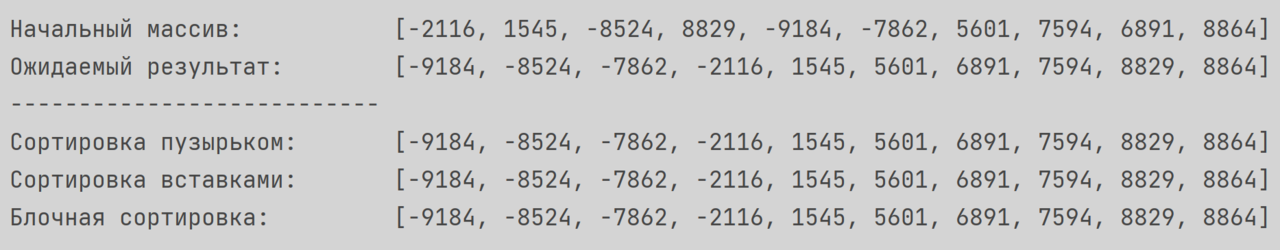
\includegraphics[width=480pt]{inc/output.png}
	\caption{Пример работы программы}
	\label{fig:output}	
\end{figure}

\subsection{Сравнение времени работы реализаций алгоритмов} \label{time-comp"}

Для сравнения времени работы реализаций алгоритмов рассматривалось три случая:
\begin{enumerate} 
  \item отсортированный массив (лучший случай);
  \item неравномерно распределенный массив, отсортированный в обратном порядке (худший случай);
  \item массив из случайных чисел (произвольный случай).
\end{enumerate}

На рисунках \ref{fig:time-best}, \ref{fig:time-worst} и \ref{fig:time-random} приведены зависимости времени работы реализаций алгоритмов сортировки от размеров массивов на отсортированных, обратно отсортированных и случайных данных соответственно.

\begin{figure}[h!btp]
	\centering
	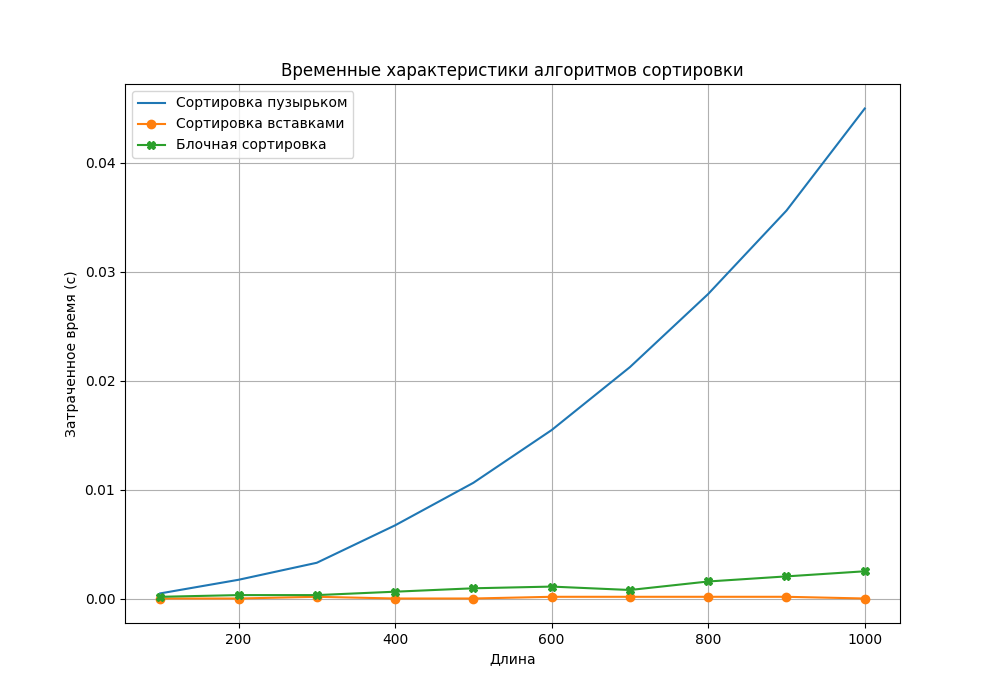
\includegraphics[width=400pt]{inc/time-best.png}
	\caption{Зависимость времени работы реализации алгоритма сортировки от размера массива для лучшего случая}
	\label{fig:time-best}	
\end{figure}
\clearpage

\begin{figure}[h!btp]
	\centering
	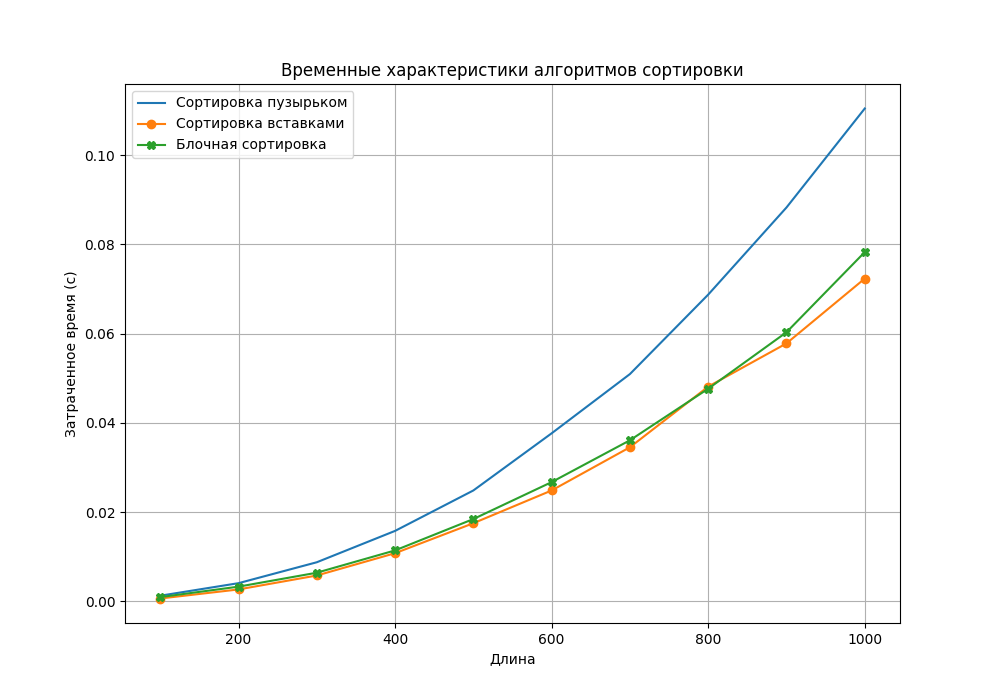
\includegraphics[width=400pt]{inc/time-worst.png}
	\caption{Зависимость времени работы реализации алгоритма сортировки от размера массива для худшего случая}
	\label{fig:time-worst}	
\end{figure}

\begin{figure}[h!btp]
	\centering
	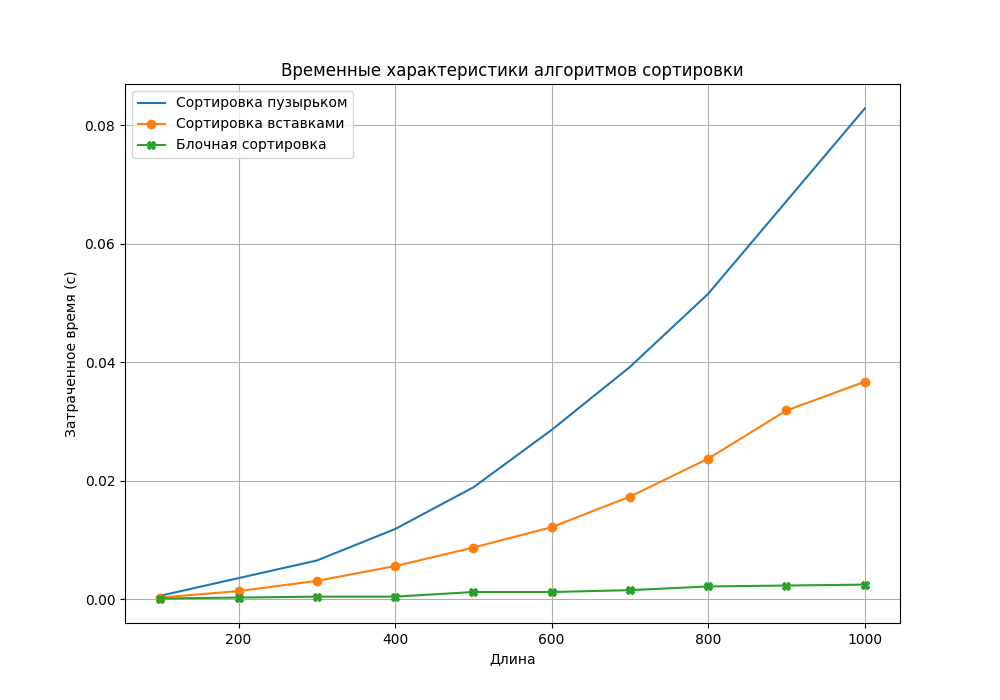
\includegraphics[width=400pt]{inc/time-random.png}
	\caption{Зависимость времени работы реализации алгоритма сортировки от размера массива для произвольного случая}
	\label{fig:time-random}	
\end{figure}
\clearpage

\subsection{Вывод}
Реализация алгоритма сортировки пузырьком является самой медленной для всех случаев. 

В случае предварительно отсортированного массива сортировка вставками превосходит другие алгоритмы, хотя блочная не сильно от нее отстает.

Для неравномерно распределенного массива, отсортированного в обратном порядке, результаты замеров для сортировки вставками и блочной сортировки практически идентичны.

На случайных данных самой быстрой является реализация алгоритма блочной сортировки.

Таким образом, подтвердились следующие оценки трудоемкости:
\begin{itemize}
  \item реализации алгоритмов сортировки вставками и блочной сортировки в лучшем случае работают на порядок быстрее реализации сортировки пузырьком;
  \item реализации алгоритмов сортировки вставками и блочной сортировки практически идентичны по времени работы в худшем случае.
\end{itemize}
